Für den Datenzugriff auf die Datenbank wurden zu jeder Collection Service-Module unter dem Verzeichnis '/services' erstellt, die entsprechenden Zugriff gewähren. Dafür wurden innerhalb der Service-Module die benötigten Zugriffsfunktionen implementiert (siehe Abbildung \ref{fig:node_service_structure}).

\begin{figure}[tbt]
\centering
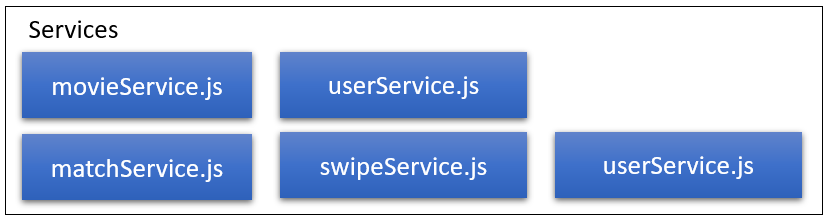
\includegraphics[width=12cm]{images/serviceStruktur.PNG}
\caption{Node.js Server - Services Struktur}
\label{fig:node_service_structure}
\end{figure}


%
%              Movie
%                   Service
%

\paragraph{Movie Service}
Die Funktionen des Moduls movieService.js bieten innerhalb der Projektumgebung den Zugriff auf bestimmte Operationen, die auf die Collection movies angewandt werden. Das Funktionsspektrum begrenzt sich für diesen Service auf die Funktion 'FindMovieExcept', die in Listing \ref{lst:findmoviesexcept} zu sehen ist.\\

\noindent
\textbf{FindMoviesExcept:}
Diese Funktion erhält als Parameter 'excludedMovies' eine Liste von MovieID's und als Parameter 'amount' einen Integerwert.
Über die Find-Funktion des importierten Movie-Models wird eine über den Wert von 'amount' begrenzte Anzahl an Movie-Dokumenten ausgelesen, deren IDs nicht in der übergebenen 'excludedMovies'-Liste vorhanden sind. Für das Filtern wird die 'nin'-Operation verwendet\footnote{Siehe Dokumentation: \url{https://docs.mongodb.com/manual/reference/operator/query/nin/}, letzter Zugriff: 26. April 2021}.\\
Sollte die Datenbank bei der Datenauslese einen Fehler zurückgeben, wird dieser über den try-catch-Block gefangen und an im Aufrufstack liegende Funktion über das Schlüsselwort throw weitergeleitet.\\

\begin{lstlisting}[caption=movieService.js - FindMoviesExcept, label=lst:findmoviesexcept]
const Movie = require('../database/models/movie')

async function FindMoviesExcept(excludedMovies, amount) {
    var movies;

    try{ 
    movies = await Movie.find({ id: { $nin: excludedMovies }}).limit(amount); }
    }
    catch(err){throw err;}

    return movies;
}

module.exports.FindMoviesExcept = FindMoviesExcept;
\end{lstlisting}


%
%              User
%                   Service
%

\paragraph{User Service}
Die Funktionen des Moduls userService.js bieten innerhalb der Projektumgebung den Zugriff auf bestimmte Operationen, die auf die Collection User angewandt werden. Dieser Service import das User-Model.\\

\noindent
\textbf{CreateUser:}
Die in Listing \ref{lst:userservicecreateuser} dargestellte Funktion erhält sämtliche Eigenschaften, die im User-Schema beschrieben sind, als Parameter. Diese Funktion wird in der Projektumgebung in Zusammenhang mit mindestens einer weiteren datenbankzugreifenden Funktion aufgerufen. Im Sinne einer Transaktion müssen sie als atomare Operationen ausgeführt werden, um den Datenbestand konsistent zu halten. Daher wird ein Session-Objekt als Parameter mitgeliefert. Innerhalb der Funktion wird über die Create-Funktion des importierten User-Models ein neuer Eintrag in der User-Collection der Datenbank erstellt.\\

\begin{lstlisting}[caption=User Service - CreateUser, label=lst:userservicecreateuser]
async function CreateUser(uid, swipeid, matchid, city, malewanted, femalewanted, diversewanted, mygender, session) {
    try {
        return (await User.create([{
            _id: mongoose.Types.ObjectId(),
            uid: uid,
            _swipeid: swipeid,
            _matchid: matchid,

            city: city,
            malewanted: malewanted,
            femalewanted: femalewanted,
            diversewanted: diversewanted,
            mygender: mygender
        }
        ], { session: session }))[0];
    }
    catch (Exception) {
        throw Exception;
    }
}
\end{lstlisting}

\noindent
\textbf{CheckExistence:}
Wie in Listing \ref{lst:userservicecheckexistence} zu sehen prüft diese Funktion, ob innerhalb der User-Collection ein User mit entsprechendem Wert für die Eigenschaft 'uid', die als Parameter übergeben wird, existiert und gibt entsprechend den boolschen Wert 'true' bei Vorhandensein beziehungsweise 'false' bei Nicht-Vorhandensein zurück.\\

\begin{lstlisting}[caption=User Service - CheckExistence, label=lst:userservicecheckexistence]
async function CheckExistence(uid) {
    return await User.exists({ uid: uid });
}
\end{lstlisting}

\noindent
\textbf{GetCityFromUser:}
Diese Funktion gibt den Eintrag der Eigenschaft 'city' eines Dokuments zurück, dessen 'uid'-Attribut mit dem übergebenen 'uid'-Parameter übereinstimmt, wie in Listing \ref{lst:userservicecheckexistence} zu sehen ist.\\

\begin{lstlisting}[caption=User Service - CheckExistence, label=lst:userservicecheckexistence]
async function GetCityFromUser(uid) {
    try {
        var user = await User.findOne({ 'uid': uid });
        if (user) {
            return user.city;
        }
        else throw { message: "No user Found" + uid };
    }
    catch (err) { console.log(err); throw err; }
\end{lstlisting}

\noindent
\textbf{ChangeCityFromUser:}
Die in Listing \ref{lst:userservicechangecityfromuser} dargestellte Funktion führt ein Update auf einem User-Dokument aus, dessen 'uid'-Eigenschaft mit dem gleichnamigen übergebenem Parameter übereinstimmt. Dabei wird die 'city'-Eigenschaft innerhalb des User-Dokuments auf den Wert des gleichnamigen Parameters aktualisiert.\\

\begin{lstlisting}[caption=User Service - ChangeCityFromUser, label=lst:userservicechangecityfromuser]
async function ChangeCityFromUser(uid, city, session) {  
   try {
        if (CheckExistence(uid)) {
            await user.UpdateOne(
                { 'uid': uid },
                { city: city },
                { session: session });
        }
        else throw { message: "No User Found" + uid }
    }
    catch (err) { console.log(err); throw err; }
\end{lstlisting}

\noindent
\textbf{ChangeGenderWantedFromUser:}
Diese Funktion erfüllt die gleiche Funktionalität wie die ChangeCityFromUser-Funktion  mit dem Unterschied, dass statt der 'city'-Eigenschaft die Eigenschaften 'malewanted','femalewanted' und 'diverswanted' aktualisiert werden.\\

\noindent
\textbf{ChangeGenderFromUser:}
Die Funktion ChangeGenderFromUser erfüllt die gleiche Funktionalität wie die ChangeCityFromUser-Funktionalität mit dem Unterschied, dass statt der 'city'-Eigenschaft die 'mygender'-Eigenschaft aktualisiert wird.\\


%
%              Match
%                   Service
%


\paragraph{Match Service}
Die Funktionen des Moduls matchService.js bieten innerhalb der Projektumgebung den Zugriff auf bestimmte Operationen, die auf die Collection matches angewandt werden. Dieser Service import das Match-Model.

\noindent
\textbf{CreateUserMatchDocument:}
Die in Listing \ref{lst:matchserviceCreateUserMatchDocument} dargestellte Funktion überprüft zunächst, ob ein Match-Dokument mit übergebener 'uid'-Eigenschaft bereits existiert. Ist dies nicht der Fall, wird ein neues Match-Dokument in der matches-Collection erzeugt.\\

\begin{lstlisting}[caption=Match Service - CreateUserMatchDocument, label=lst:matchserviceCreateUserMatchDocument]
async function CreateUserMatchDocument(uid, session) {
    if (!(await Match.exists({ uid: uid }))) {
        try {
            return (await Match.create([{
                _id: mongoose.Types.ObjectId(),
                uid: uid,
                swipes: []}
            ], { session: session }))[0];
        }
        catch (Exception) {
            throw Exception;
        }
    }
    else 
      throw { message: "Match already exists for " + uid 		};
    
}
\end{lstlisting}

\noindent
\textbf{CheckMatchExists:}
Wie in Listing \ref{lst:matchserviceCreateUserMatchDocument} zu sehen, überprüft diese  Funktion ob ein Match-Dokument existiert, welches den übergebenen 'uid'-Eigenschaftswert hat sowie innerhalb seiner 'supermatches'- oder 'normalmatches'-Liste die übergebene 'matchedUid' enthält. Zurück wird ein entsprechender boolescher Wert geschickt. \\

\begin{lstlisting}[caption=Match Service - CreateUserMatchDocument, label=lst:matchserviceCreateUserMatchDocument]
async function CheckMatchExists(uid, matchedUid, session) {
    try {
        var match = await Match.findOne({ uid: uid, 'supermatches.uid': matchedUid }).session(session)

        if (match) { return true; }
        else {
            var match = await Match.findOne({ uid: uid, 'normalmatches.uid': matchedUid }).session(session)

            if (match) return true;
            else return false;
        }
    }
    catch (err) { console.log(err); throw err; }
}
\end{lstlisting}

\noindent
\textbf{AddNormalMatchToUser:}
Die Funktion AddNormalMatchToUser, welche in Listing \ref{lst:matchserviceAddNormalMatchToUser} zu sehen ist,  fügt der 'normalmatches'-Liste eines Match-Dokuments ein neues Objekt mit den Eigenschaften 'uid','matchUid' und 'movieid', die ihren Wert über die übergebenen Funktionsparameter erhalten. Des Weiteren wird das Attribut 'startedChat' und 'removed' jeweils mit dem booleschen Standardwert 'false' hinzugefügt. Außerdem wird die Eigenschaft 'newChanges' des Match-Dokuments auf true gesetzt.\\

\begin{lstlisting}[caption=Match Service - AddNormalMatchToUser, label=lst:matchserviceAddNormalMatchToUser]
async function AddNormalMatchToUser(uid, matchedUid, movieid, session) {
 try {
  if (Match.exists{ 'uid': uid }) {
   await Match.findOneAndUpdate(
    { 'uid': uid },
    { newChanges: true,
    $push: { normalmatches: { uid: matchedUid, 
                              movieid: movieid, 
                              startedChat: false, 
                              removed: false } }},
    { session: session });
    } else throw { message: "No Match Found" }; }
    catch (err) { console.log(err); throw err; }
}
\end{lstlisting}

\noindent
\textbf{AddSuperMatchToUser:}
Die Funktion unterscheidet sich von 'AddNormalMatchToUser' nur in dem Aspekt, dass ein neuer Eintrag in die 'supermatches'- statt der 'normalmatches'-Liste hinzugefügt wird.\\

\noindent
\textbf{GetMatches:}
Die Funktion empfängt eine 'uid' als Parameter und gibt ein entsprechendes Match-Dokument zurück, sofern es existiert.\\

\noindent
\textbf{SuperMatchMarkAsRemoved:}
Innerhalb der Funktion wird, wie in Listing \ref{lst:matchserviceSuperMatchMarkAsRemoved} dargestellt, anhand des übergebenen 'uid' und 'matchesUid' der Eintrag in der 'supermatches'-Liste angepasst. Dabei wird der Wert für 'removed' auf true gesetzt. Ausserdem wird 'newChanges' des betroffenen Match-Dokuments auf true gesetzt.\\

\begin{lstlisting}[caption=Match Service - SuperMatchMarkAsRemoved, label=lst:matchserviceSuperMatchMarkAsRemoved]
async function SuperMatchMarkAsRemoved(uid, matchUid, session) {
 try {
  var match = await Match.findOneAndUpdate({ uid: uid, "supermatches.uid": matchUid },
  { "$set": { newChanges: true,
             "supermatches.$.removed": true }},
            { session: session });
  if (!match) {
   throw { message: "No Match Found:" + 
           uid + "matching: " + matchUid };}
 } catch (err) { console.log(err); throw err; }
}
\end{lstlisting}

\noindent
\textbf{NormalMatchMarkAsRemoved:}
Die Funktion unterscheidet sich von 'SuperMatchMarkAsRemoved' nur in dem Aspekt, dass der  Eintrag in der 'supermatches'- statt der 'normalmatches'-Liste angepasst wird.\\

\noindent
\textbf{MatchesReceived:}
Anhand einer übergebenen 'uid' und 'matchUid' wird die Eigenschaft 'new"-Changes' eines entsprechenden Match-Dokuments in der Match-Collection auf den booleschen Wert false gesetzt. 



%
%              Swipe
%                   Service
%

\paragraph{Swipe Service}
Die Funktionen des Moduls swipeService.js bieten innerhalb der Projektumgebung den Zugriff auf bestimmte Operationen, die auf die Collection swipes angewandt werden. Dieser Service importiert das Swipe-Model.\\

\noindent
\textbf{CreateUserSwipeDocument:}
Die Funktion erfüllt die gleiche Funktionalität wie die 'Create\-UserMatchDocument'-Funktionalität des Match-Services mit dem Unterschied, dass anstelle eines Match-Dokuments ein Swipe-Dokument in der swipes-Collection erstellt wird.\\

\noindent
\textbf{AddSwipe:}
Die in Listing \ref{lst:swipeserviceaddswipe} dargestellte Funktion erstellt zunächst ein 'swipe'-Objekt mit den Eigenschaften 'movieid' und 'swipeaction' und entnimmt die Werte dafür aus den gleichnamigen übergebenen Parametern. 
Wenn ein Swipe-Dokument mit übergebener 'uid' existiert, wird überprüft ob das Dokument in der 'swipes'-Liste bereits ein Eintrag mit entsprechender movieid enthält. Ist dies der Fall, wird die 'swipeaction'-Eigenschaft auf den Wert des übergebenen gleichnamigen Parameters aktualisiert. Ansonsten wird der Liste das zu Beginn erstellte 'swipe'-Objekt hinzugefügt. Letzlich wird das Swipe-Dokument über die Save-Funktion des Save-Models gespeichert.\\

\begin{lstlisting}[caption=Swipe Service - AddSwipe, label=lst:swipeserviceaddswipe]
async function AddSwipe(uid, movieid, swipeaction) {
 var swipe = { movieid: movieid, swipeaction: swipeaction };
 var dbSwipe;
 if (Swipe.exists({ 'uid': uid })) {
  try {
   dbSwipe = await Swipe.findOne({ 'uid': uid });

   //Ueberpruefe Vorhandensein des Swipes
   var index = dbSwipe.swipes.findIndex(x => x.movieid === movieid);

   if (index >= 0) {
    if (dbSwipe.swipes[index].swipeaction != swipeaction)
      dbSwipe.swipes[index].swipeaction = swipeaction; }
    else { dbSwipe.swipes.push(swipe); }
    dbSwipe.save(); 
    } catch (err) { throw err; }
  } else { throw "No Swipe available for this uid " + uid;}
  dbSwipe.save();
  return swipe;
}
\end{lstlisting}

\noindent
\textbf{RequestSwipes:}
Die Funktion empfängt eine 'uid' als Parameter und gibt ein entsprechendes Match-Dokument zurück, sofern es existiert.\\

\noindent
\textbf{RequestSuperlikeSwipes:}
Innerhalb dieser in Listing \ref{lst:swipeserviceRequestSuperlikeSwipes} dargestellten Funktion kommt es zum Einsatz einer Aggregation. 
Dabei kommt es zum Einsatz mehrerer Pipeline-Operatoren.
% %TODO Link auf Tabelle 5 Aggregation Framework
Über den 'unwind'-Operator wird gesetzt, dass für jeden Listeneintrag innerhalb der 'swipes'-Liste neue Dokumente erzeugt werden, die in die nachfolgende Pipeline-Stufen weitergeleitet werden. Anhand des 'match'-Operators werden dann die neuen Dokumente gefiltert. Letztlich wird eine Liste von Swipes zurückgeschickt, die eine 'swipeaction' von 2 (repräsentativ für Superlike) aufweisen.\\

\begin{lstlisting}[caption=Swipe Service - RequestSuperlikeSwipes, label=lst:swipeserviceRequestSuperlikeSwipes]
async function RequestSuperlikeSwipes(uid) {
 var dbSwipe;
 if (Swipe.exists({ 'uid': uid })) {
  try {
   dbSwipe = await (await Swipe.aggregate([
    { $unwind: '$swipes' },
    { $match: { uid: uid,
                'swipes.swipeaction': 2 }},
    { $group: { _id: '$_id',
                swipes: { $push: { movieid: "$swipes.movieid",
                                  swipeaction: "$swipes.swipeaction" 
     }}}}]));
   if (dbSwipe.length > 0 && dbSwipe[0]) {
    return dbSwipe[0].swipes; }
   } catch (err) { throw err; } }
  else {throw { message: "Swipe uid not existing " + uid }; }
}
\end{lstlisting}

\noindent
\textbf{FindAllSwipedMoviesByUserID:}
Innerhalb dieser in Listing \ref{lst:swipeserviceFindAllSwipedMoviesByUserID} dargestellten Funktion werden für eine übergebene 'uid' sämtlich 'movieid's zurückgeben, die in der 'swipes'-Liste des entsprechenden Swipe-Dokuments vorhanden sind.\\

\begin{lstlisting}[caption=Swipe Service - FindAllSwipedMoviesByUserID, label=lst:swipeserviceFindAllSwipedMoviesByUserID]
var swipedMovieIDs = [];
    
if (Swipe.exists({"uid": uid)) {
 try { var dbSwipe = await FindOne(uid);
  await dbSwipe.swipes.forEach(x => swipedMovieIDs.push(x.movieid));
 } catch (err) { throw err; }}
return swipedMovieIDs;
\end{lstlisting}


%
%              City
%                   Service
%
\paragraph{City Service}
Die Funktionen des Moduls cityService.js bieten innerhalb der Projektumgebung den Zugriff auf bestimmte Operationen, die auf die Collection cities angewandt werden. Dieser Service import das Swipe-Model.\\

\noindent
\textbf{GetAllInhabitedCities:}
Diese Funktion wird im Matching-Algorithmus aufgerufen. Wie in Listing \ref{lst:cityServiceGetAllInhabitedCities} zu sehen liefert er sämtliche Städte, mit mindestens zwei Nutzern. \\

\begin{lstlisting}[caption=City Service - GetAllInhabitedCities, label=lst:cityServiceGetAllInhabitedCities]
async function GetAllInhabitedCities() {
    var cities;
    try{ cities = await City.find({ user : {$exists:true},$where:'this.user.length>1'}) }
    catch (err) { throw err; }
    return cities;
}
\end{lstlisting}

\noindent
\textbf{AddUserToCity:}
Diese Funktion fügt einem 'City'-Dokument eine 'uid' hinzu.\\

\noindent
\textbf{RemoveUserFromCity:}
Diese Funktion entfernt eine 'uid' aus einem 'City'-Dokument.
